\chapter*{De Jiuzhaigou à Chengdu\markboth{De Jiuzhaigou à Chengdu}{}}
\section*{29 septembre 2015}
Jiuzhaigou est une réserve naturelle qui comprend 2 vallées avec des cascades et des lacs aux couleurs étonnantes 

 

\begin{center} 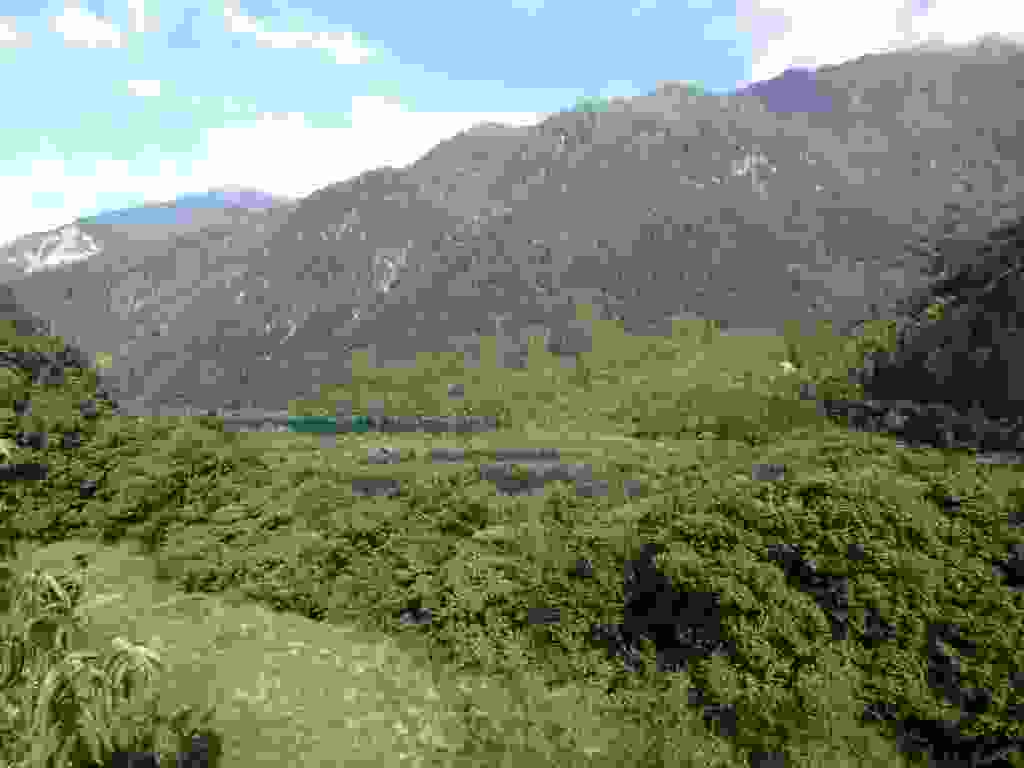
\includegraphics[width=\mywidth]{../wp-content/uploads/2015/09/P9156943-1024x768.jpg} \end{center}

 

 

\begin{center} 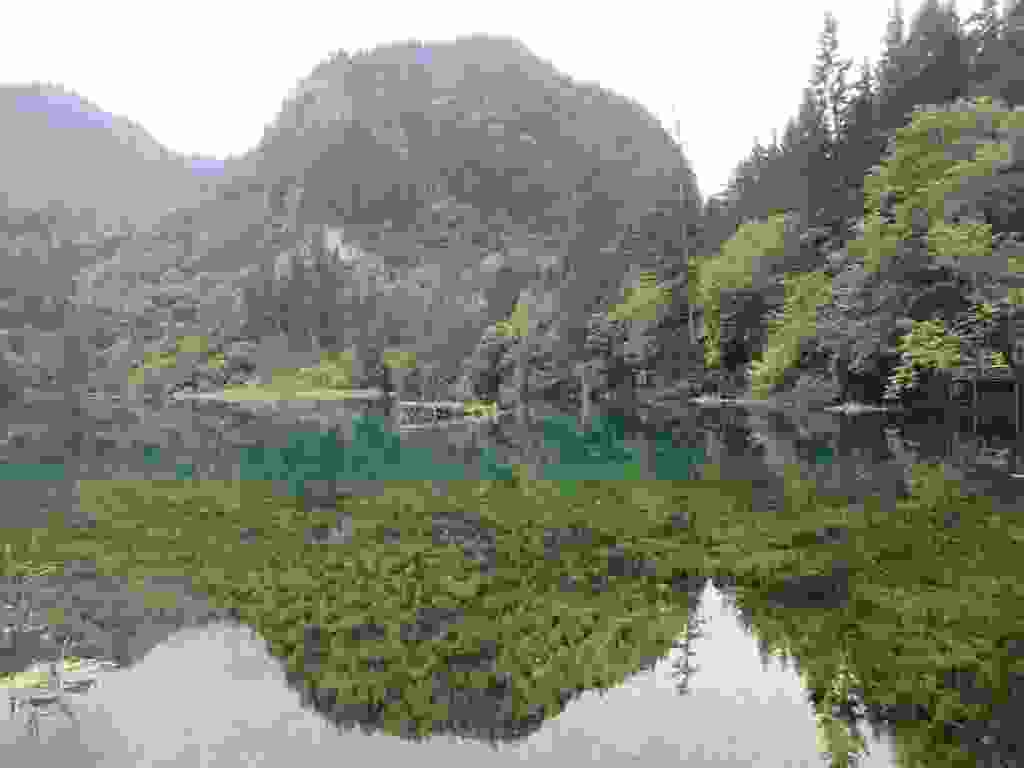
\includegraphics[width=\mywidth]{../wp-content/uploads/2015/09/P9156903-1024x768.jpg} \end{center}

 

 

\begin{center} 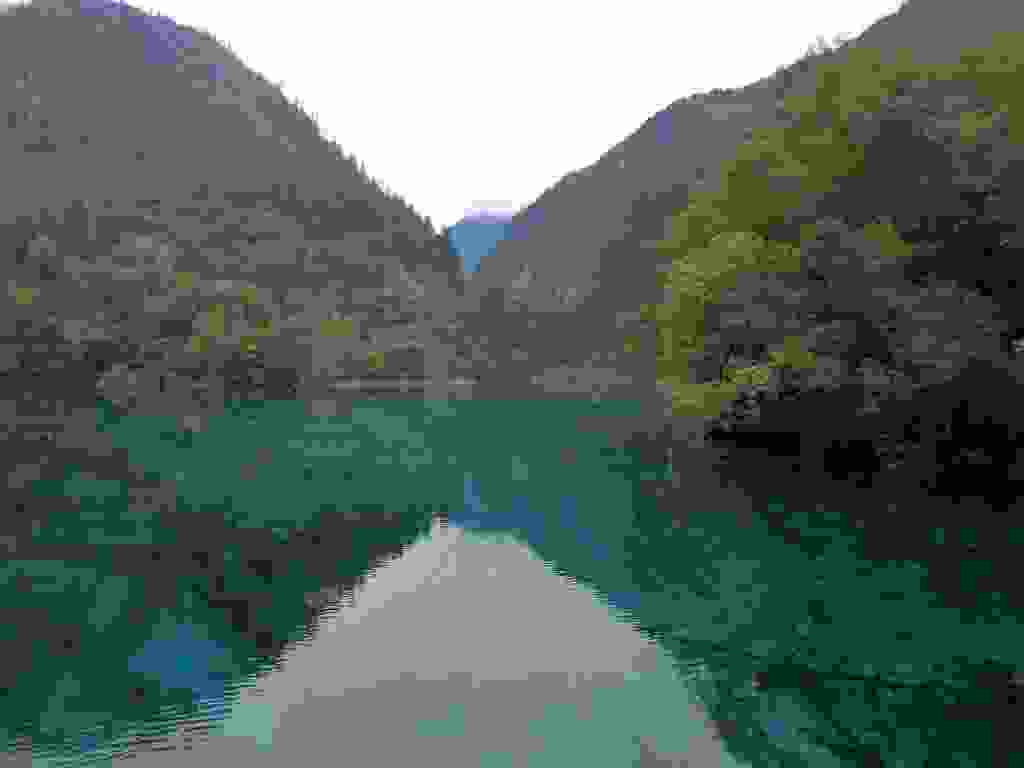
\includegraphics[width=\mywidth]{../wp-content/uploads/2015/09/P9156906-1024x768.jpg} \end{center}

 

 

\begin{center} 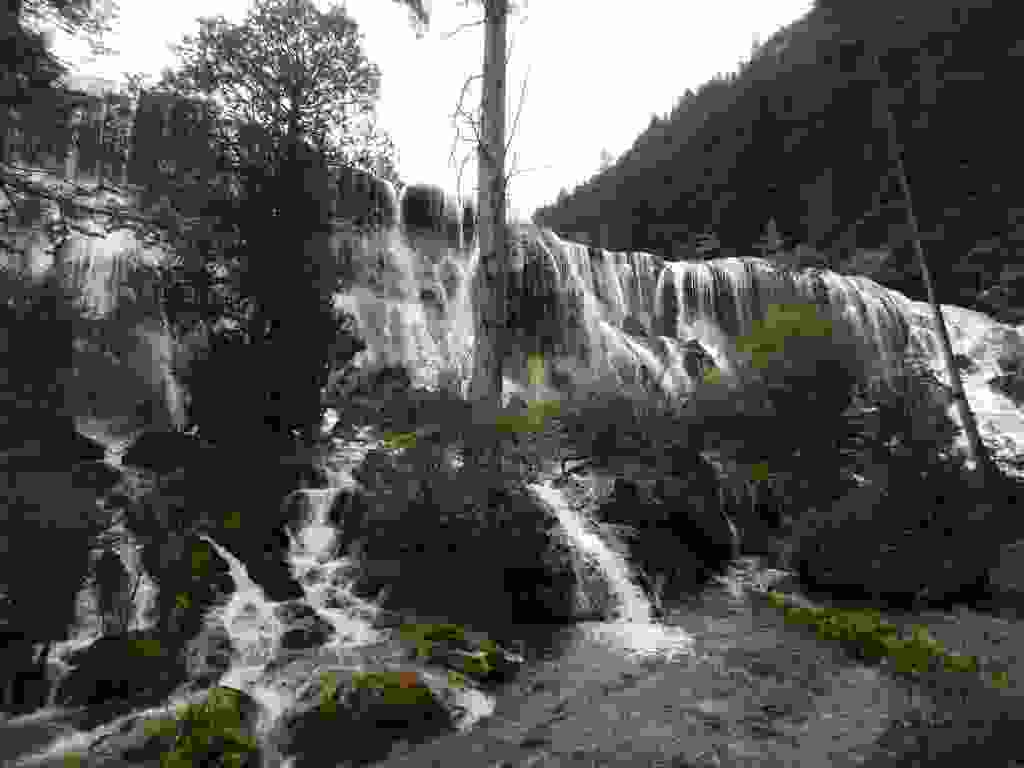
\includegraphics[width=\mywidth]{../wp-content/uploads/2015/09/P9156911-1024x768.jpg} \end{center}

 

 

\begin{center} 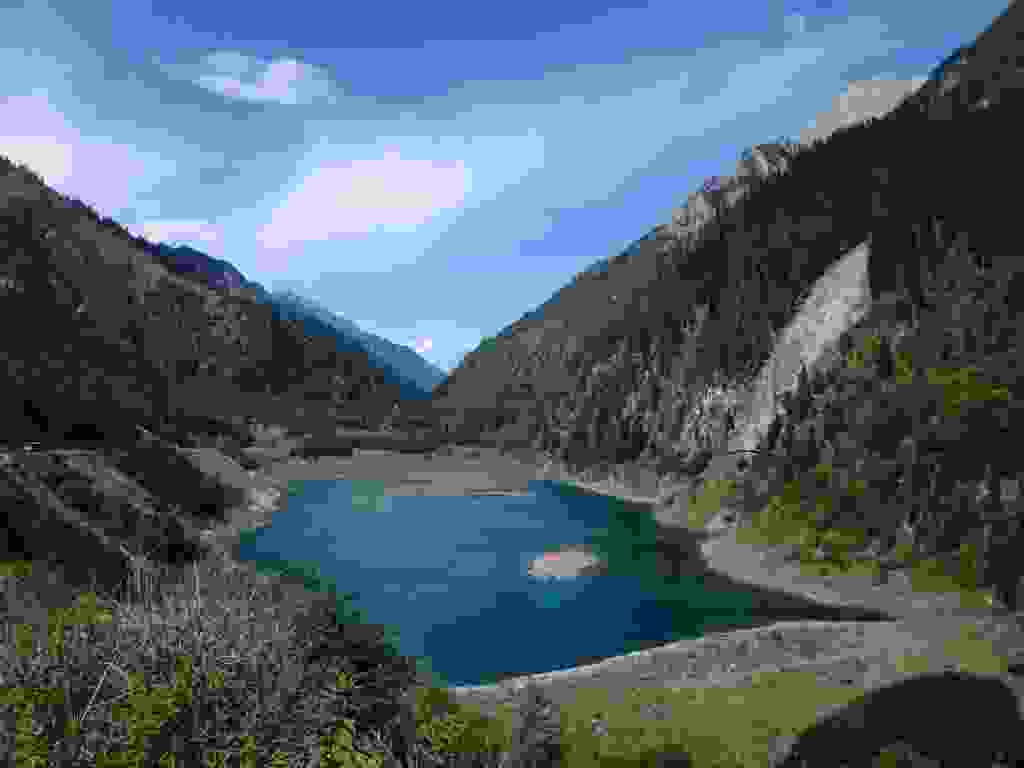
\includegraphics[width=\mywidth]{../wp-content/uploads/2015/09/P9156933-1024x768.jpg} \end{center}

 

 

\begin{center} 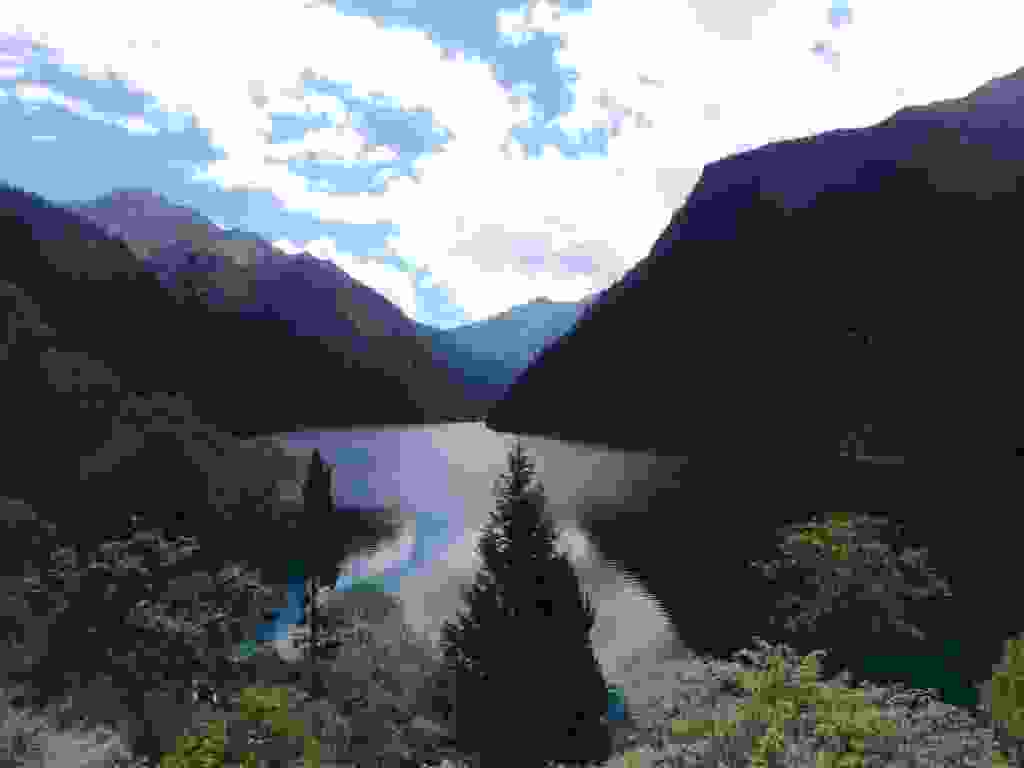
\includegraphics[width=\mywidth]{../wp-content/uploads/2015/09/P9156918-1024x768.jpg} \end{center}

 

 

\begin{center} 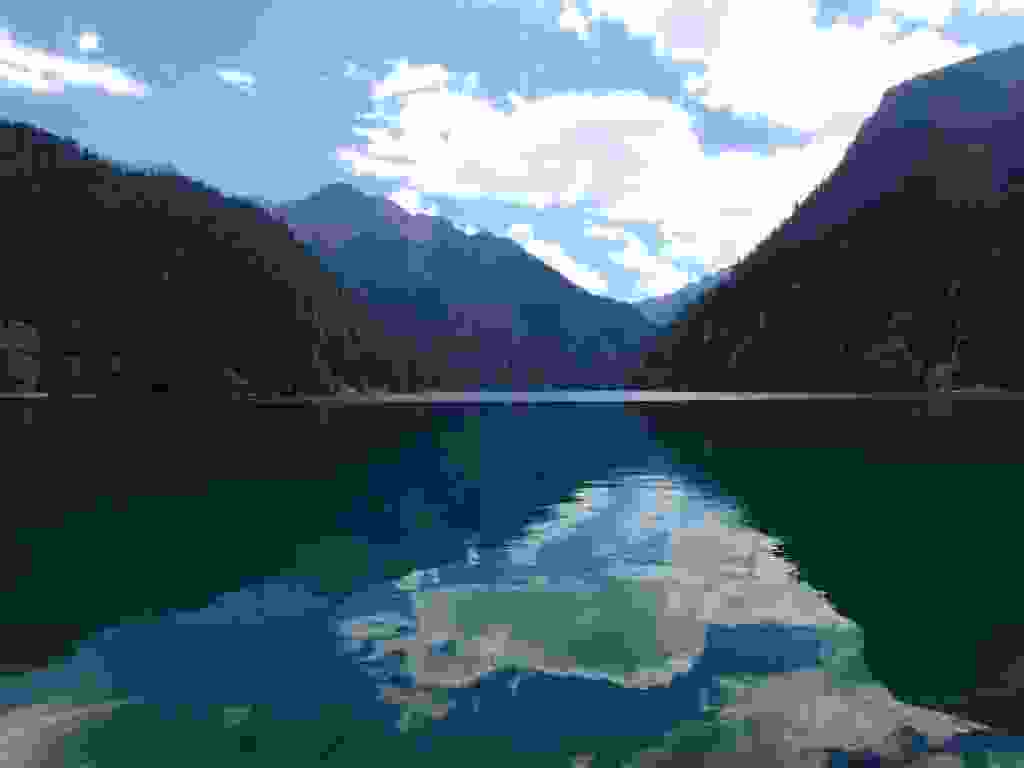
\includegraphics[width=\mywidth]{../wp-content/uploads/2015/09/P9156924-1024x768.jpg} \end{center}

 

 

\begin{center} 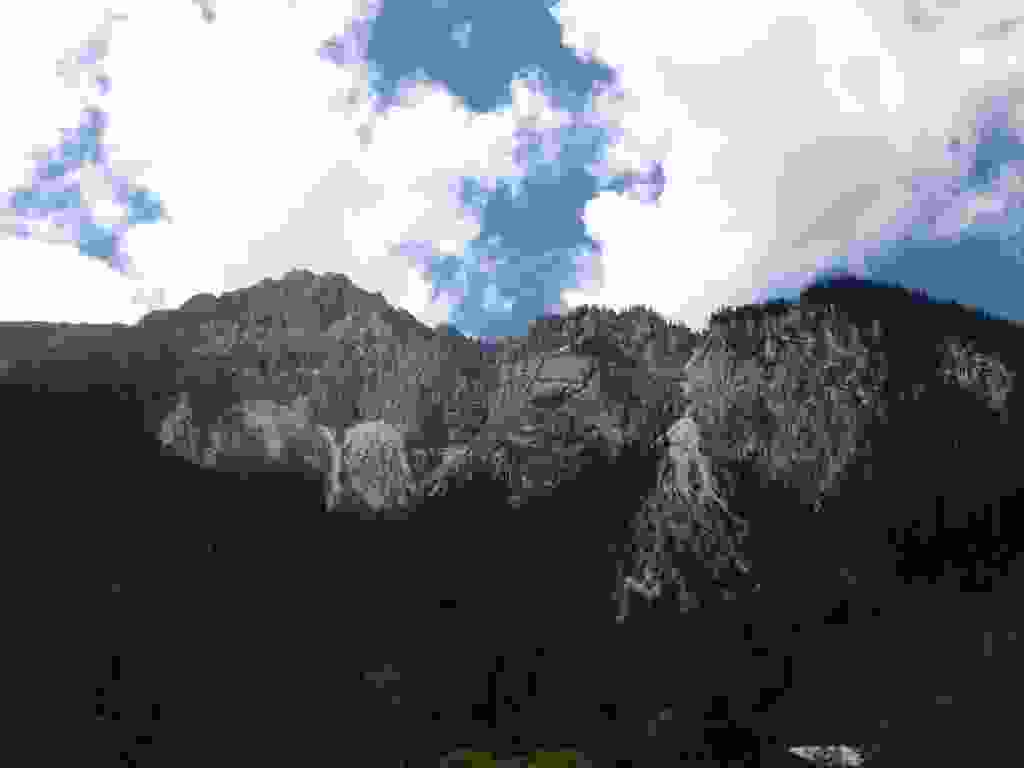
\includegraphics[width=\mywidth]{../wp-content/uploads/2015/09/P9156920-1024x768.jpg} \end{center}

 

 Le site est assez reculé dans les montagnes, pourtant des milliers de personnes le visitent chaque jour 

 

\begin{center} 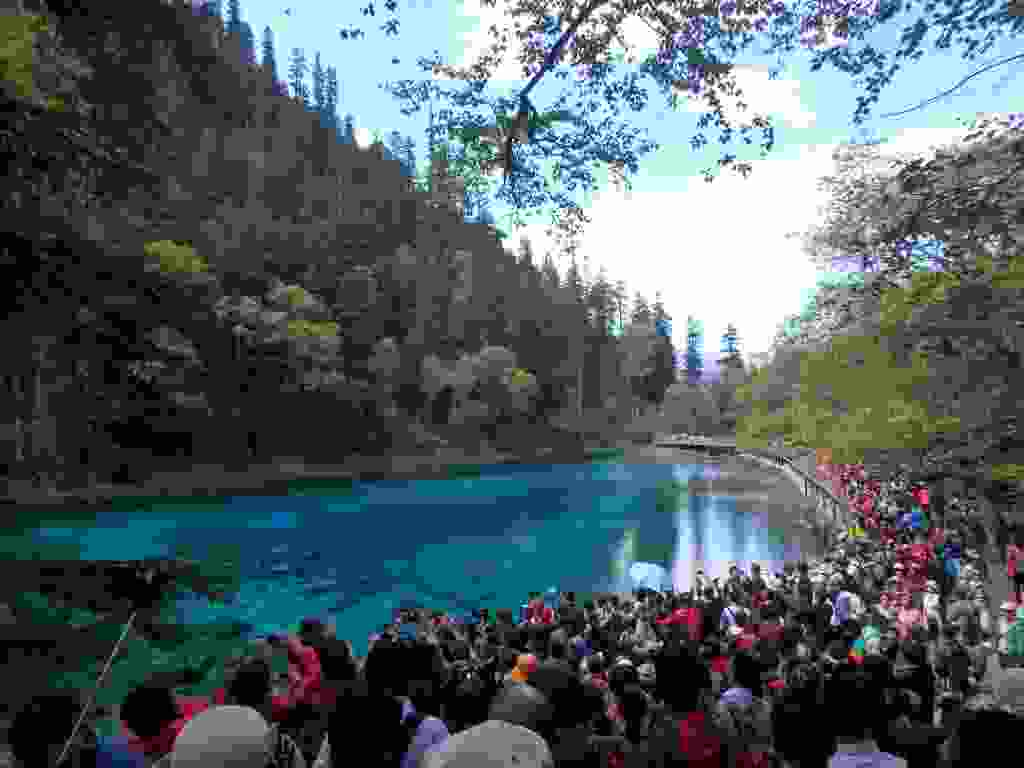
\includegraphics[width=\mywidth]{../wp-content/uploads/2015/09/P9156928-1024x768.jpg} \end{center}

 

 En partant de Jiuzhaigou, plus de 50km de montée pour entrer dans la région tibétaine d'Aba, province du Sichuan. 

 

\begin{center} 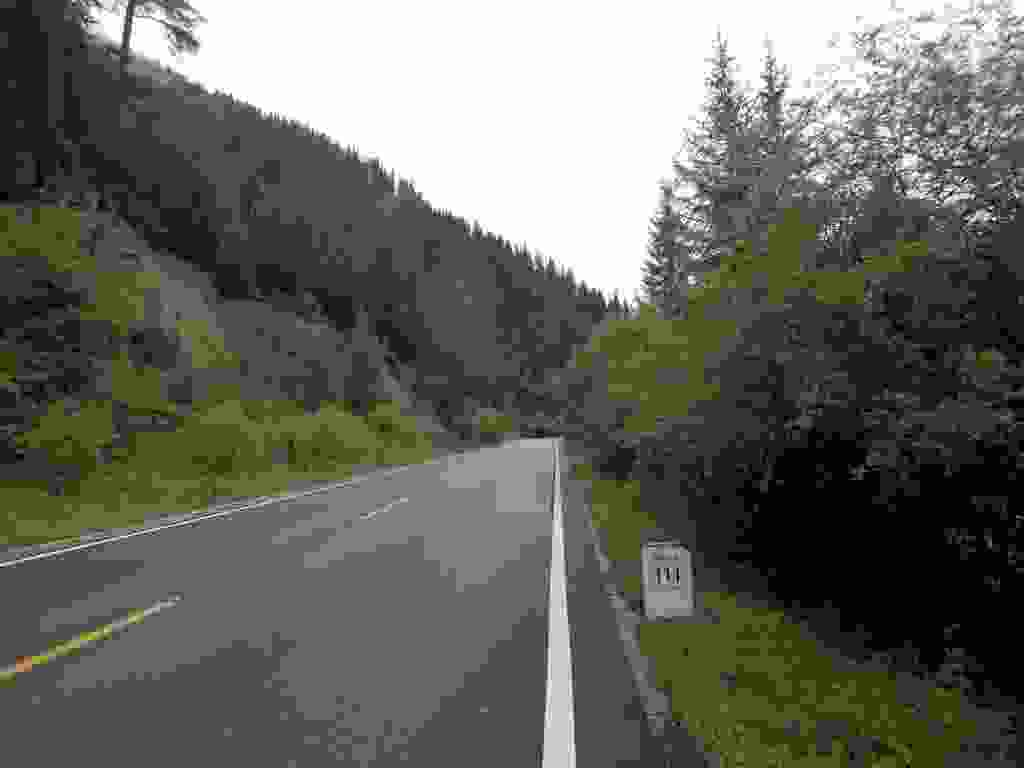
\includegraphics[width=\mywidth]{../wp-content/uploads/2015/09/wpid-p9166957-1024x768.jpg} \end{center}

 

 

\begin{center} 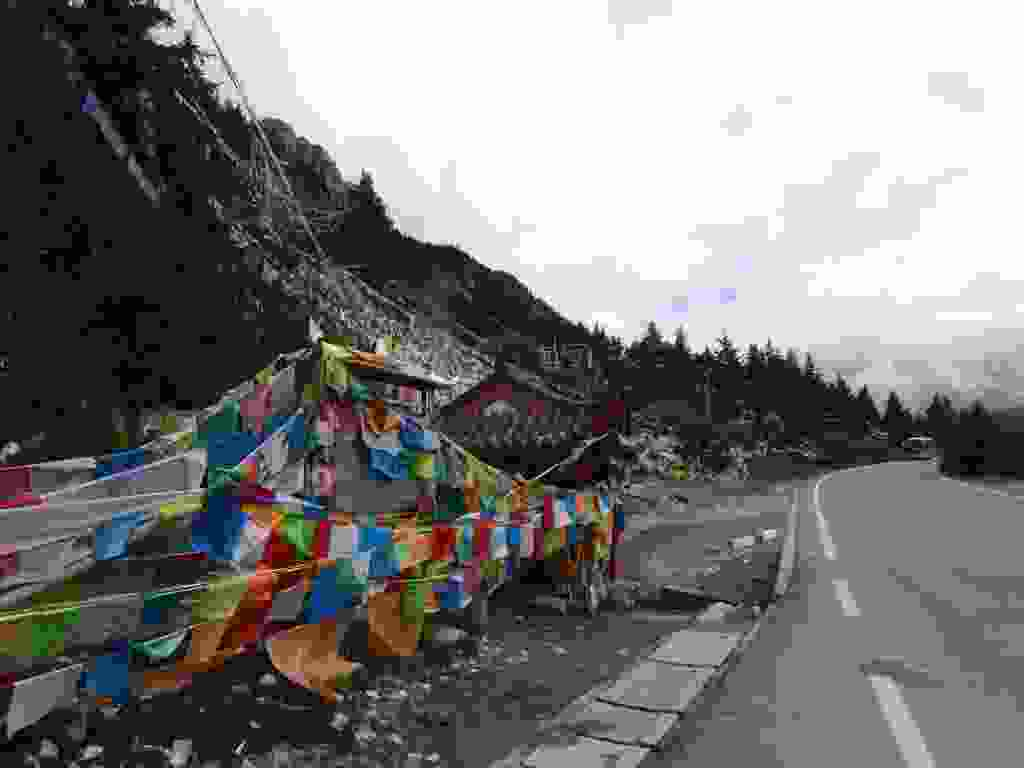
\includegraphics[width=\mywidth]{../wp-content/uploads/2015/09/wpid-p9176966-1024x768.jpg} \end{center}

 

 Restaurant bien décoré 

 

\begin{center} 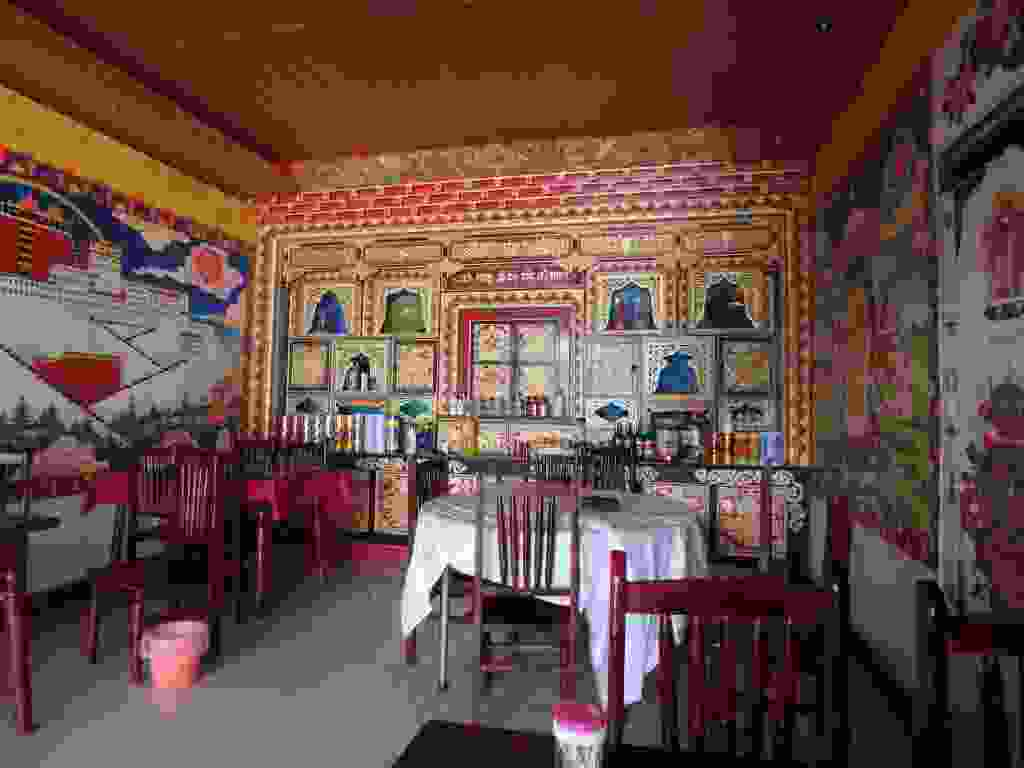
\includegraphics[width=\mywidth]{../wp-content/uploads/2015/09/P9146872-1024x768.jpg} \end{center}

 

 Temple bouddhiste et moulins à prières 

 

\begin{center} 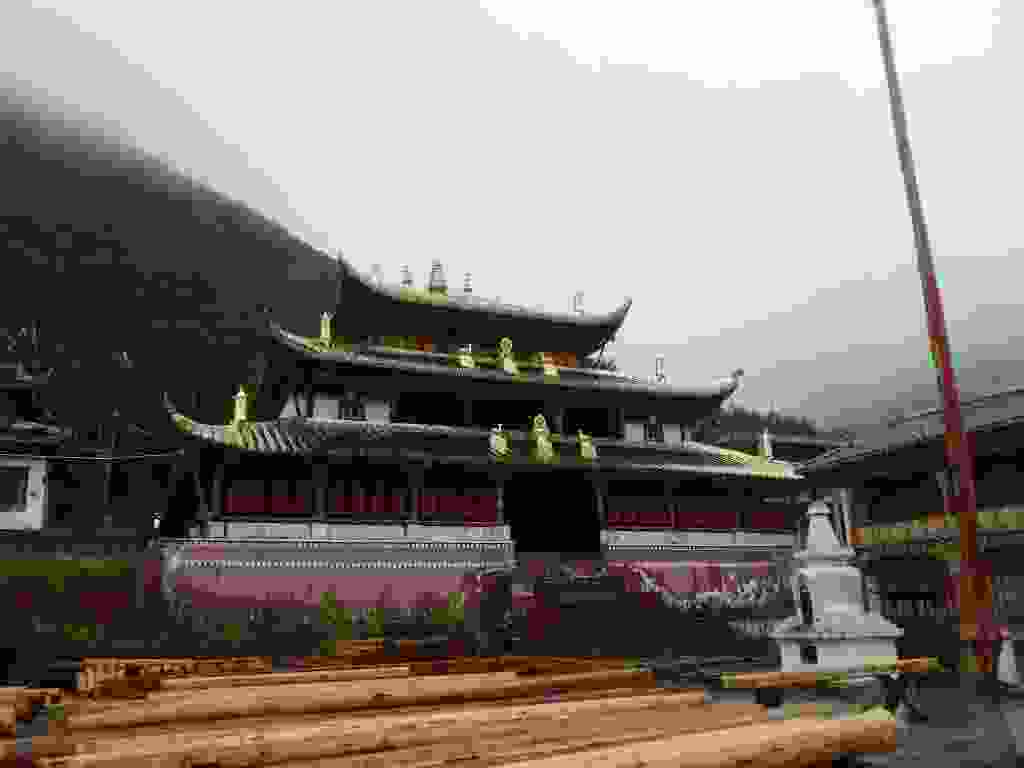
\includegraphics[width=\mywidth]{../wp-content/uploads/2015/09/wpid-p9166946-1024x768.jpg} \end{center}

 

 

\begin{center} 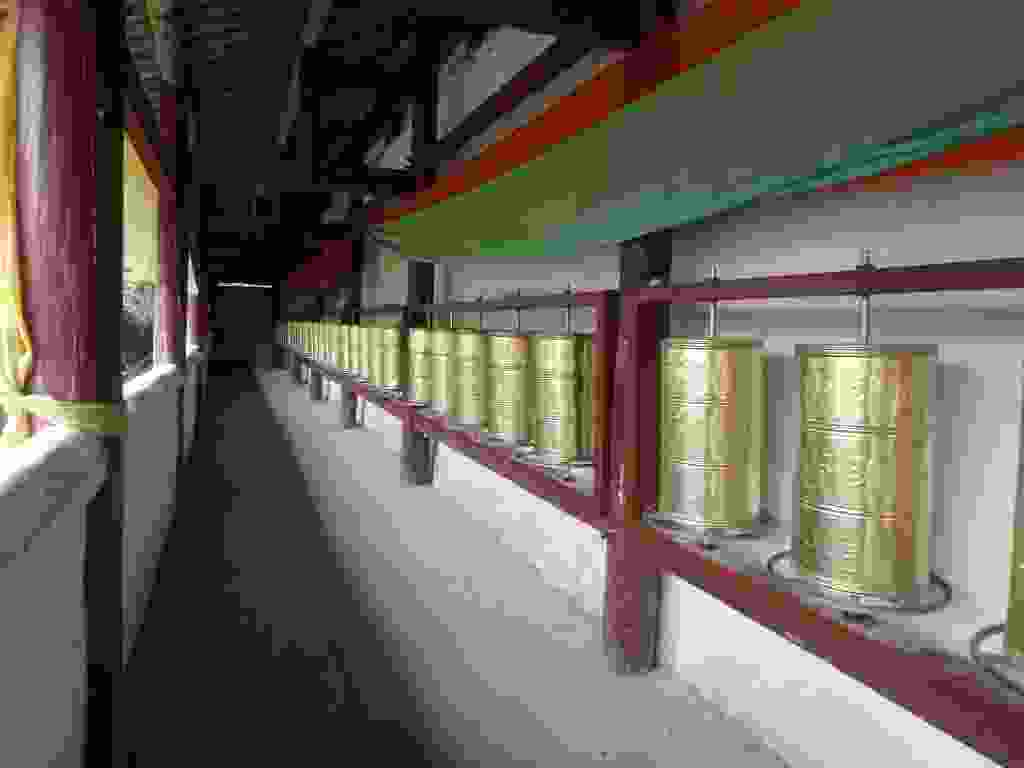
\includegraphics[width=\mywidth]{../wp-content/uploads/2015/09/wpid-p9166948-1024x768.jpg} \end{center}

 

 Troupeaux de yaks sur le plateau 

 

\begin{center} 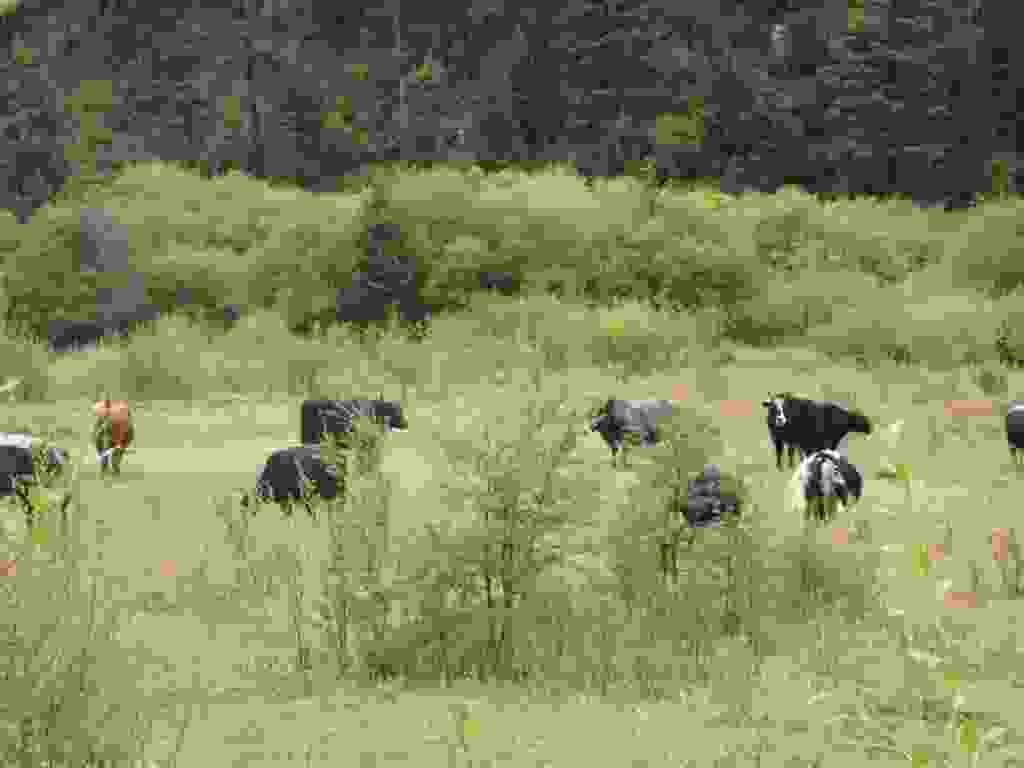
\includegraphics[width=\mywidth]{../wp-content/uploads/2015/09/wpid-p9166956-1024x768.jpg} \end{center}

 

 Après une journée complète sous la pluie je m'arrête pour boire un thé dans un petit stand. Je me retrouve invité à me réchauffer près du poêle, avec brochettes de yak, soupe et thé tibétain 

 

\begin{center} 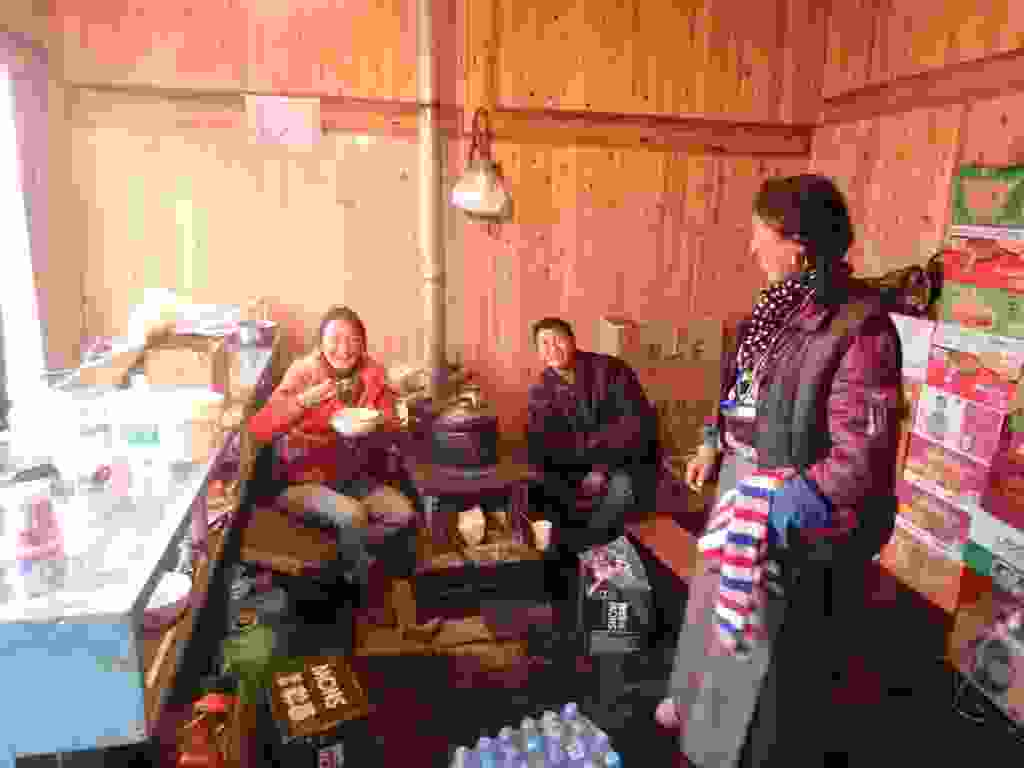
\includegraphics[width=\mywidth]{../wp-content/uploads/2015/09/wpid-p9166963-1024x768.jpg} \end{center}

 

 Les 3 journées suivantes sont en descente le long d'une rivière, en traversant des petits villages 

 

\begin{center} 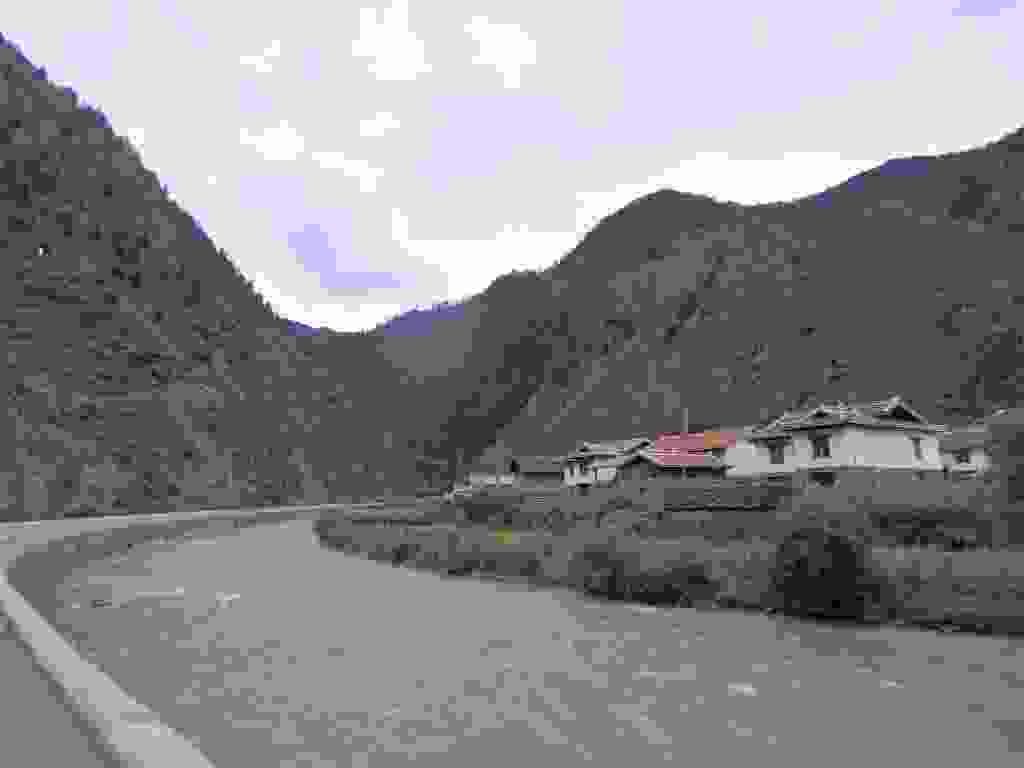
\includegraphics[width=\mywidth]{../wp-content/uploads/2015/09/wpid-p9176984-1024x768.jpg} \end{center}

 

 

\begin{center} 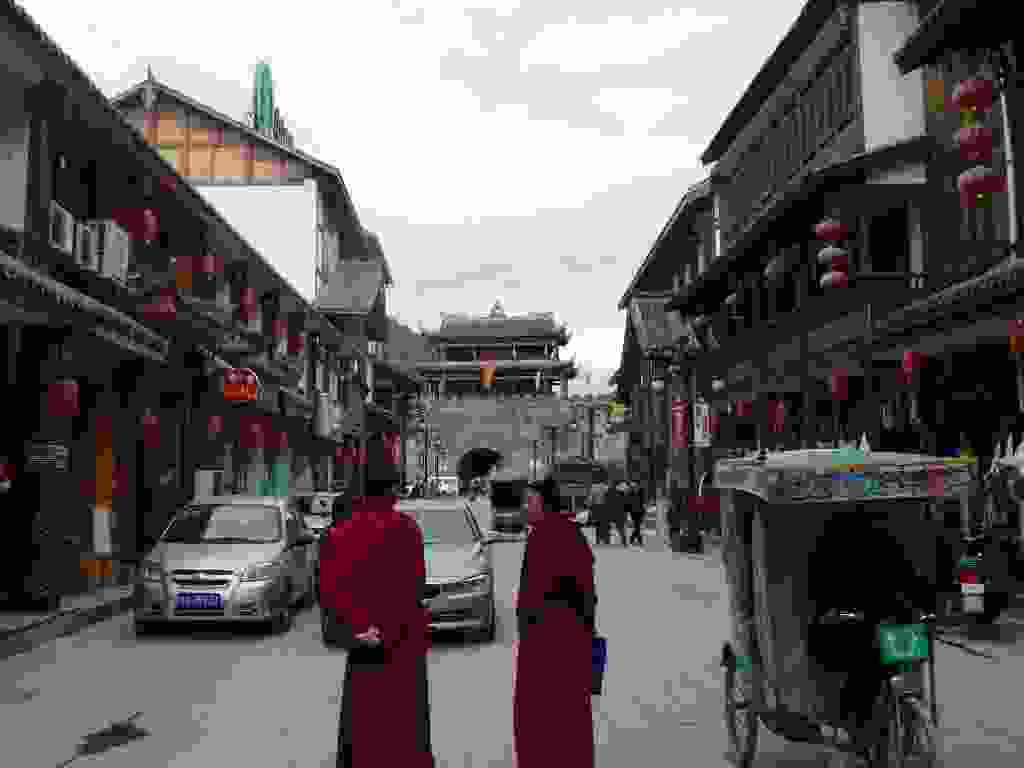
\includegraphics[width=\mywidth]{../wp-content/uploads/2015/09/wpid-p9176978-1024x768.jpg} \end{center}

 

 

\begin{center} 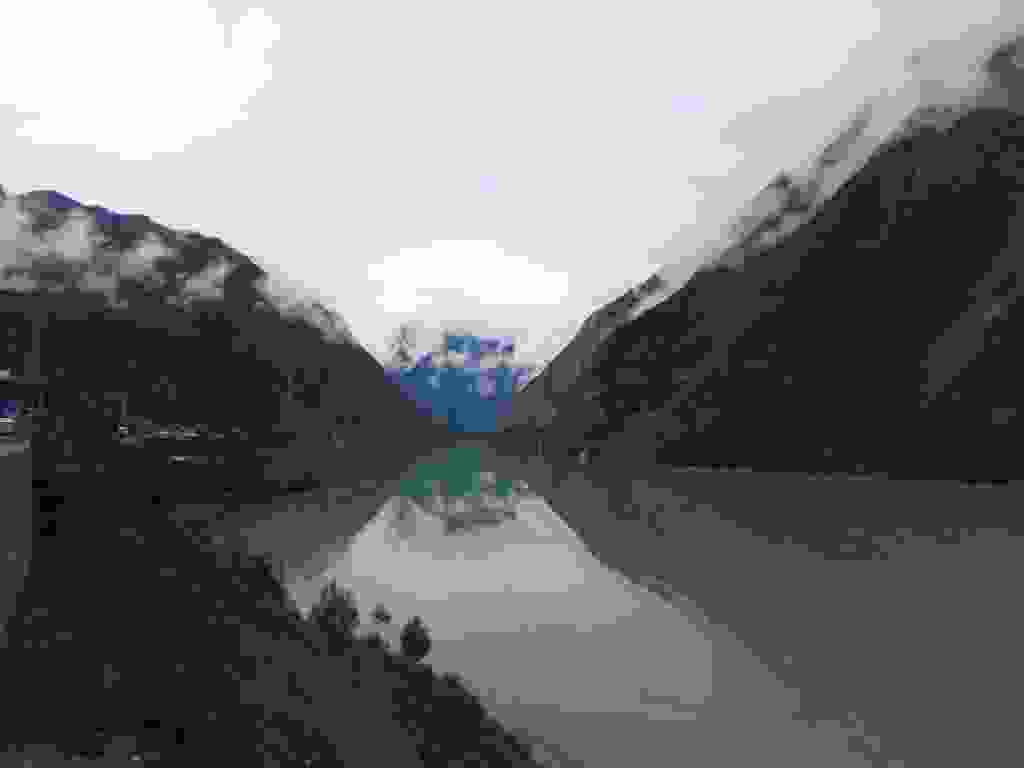
\includegraphics[width=\mywidth]{../wp-content/uploads/2015/09/wpid-p9186991-1024x768.jpg} \end{center}

 

 Un autre temple dans lequel je peux rentrer 

 

\begin{center} 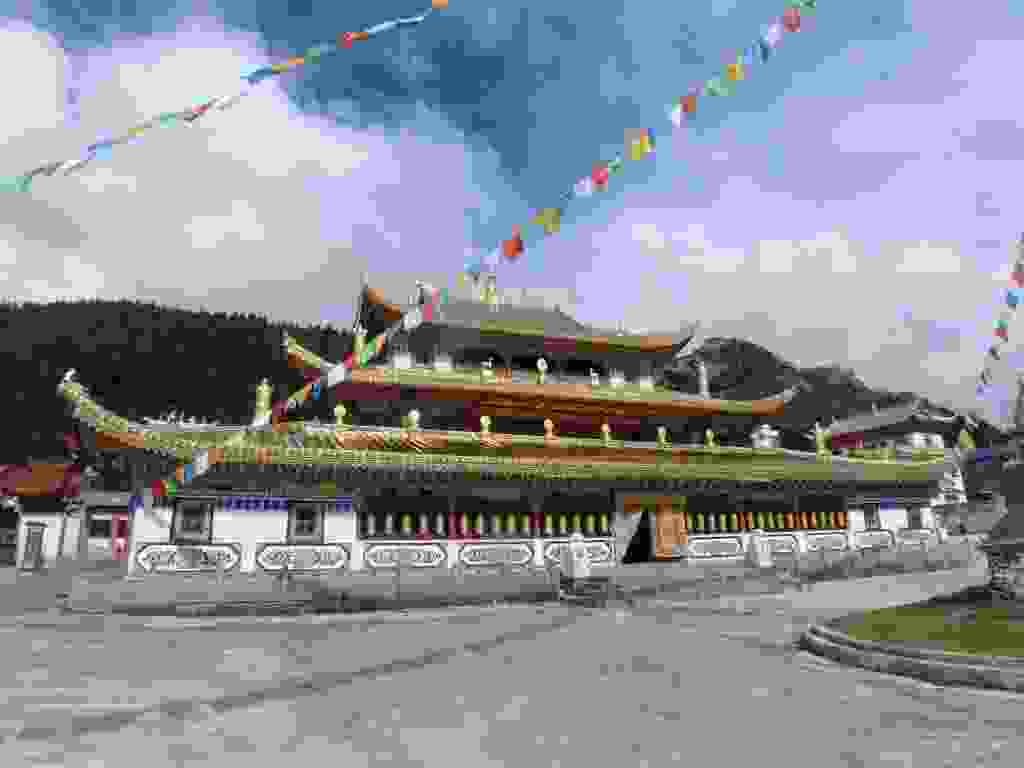
\includegraphics[width=\mywidth]{../wp-content/uploads/2015/09/wpid-p9176968-1024x768.jpg} \end{center}

 

 

\begin{center} 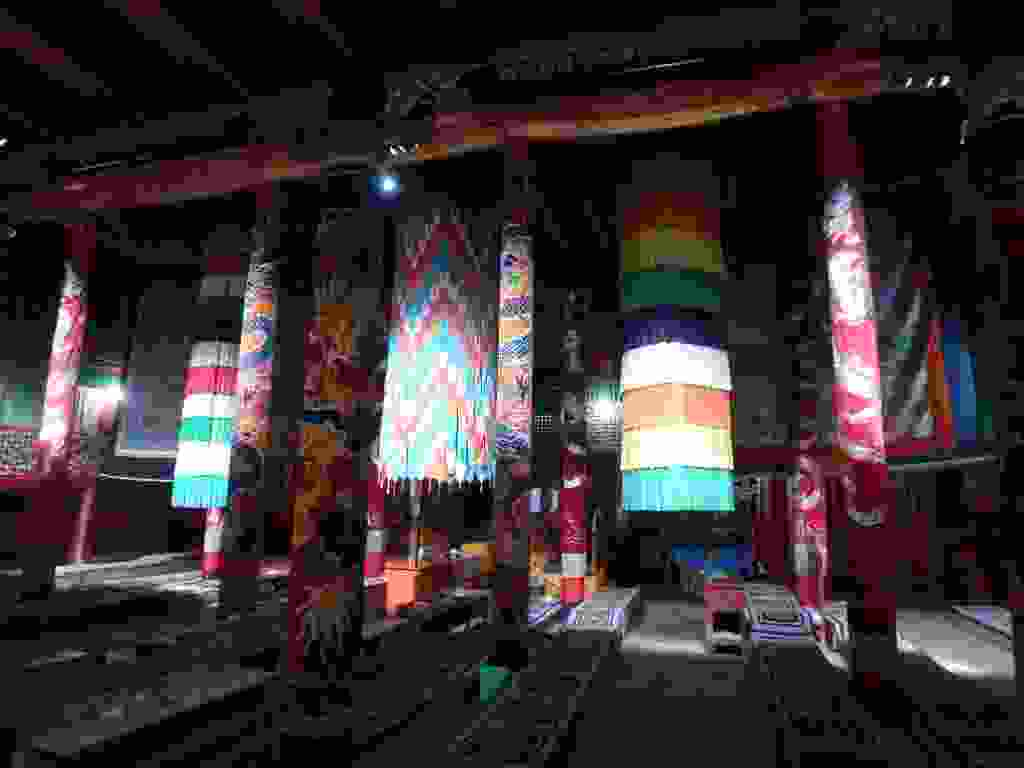
\includegraphics[width=\mywidth]{../wp-content/uploads/2015/09/wpid-p9176970-1024x768.jpg} \end{center}

 

 Trafic important avec chaque jour des centaines de bus de tourisme 

 

\begin{center} 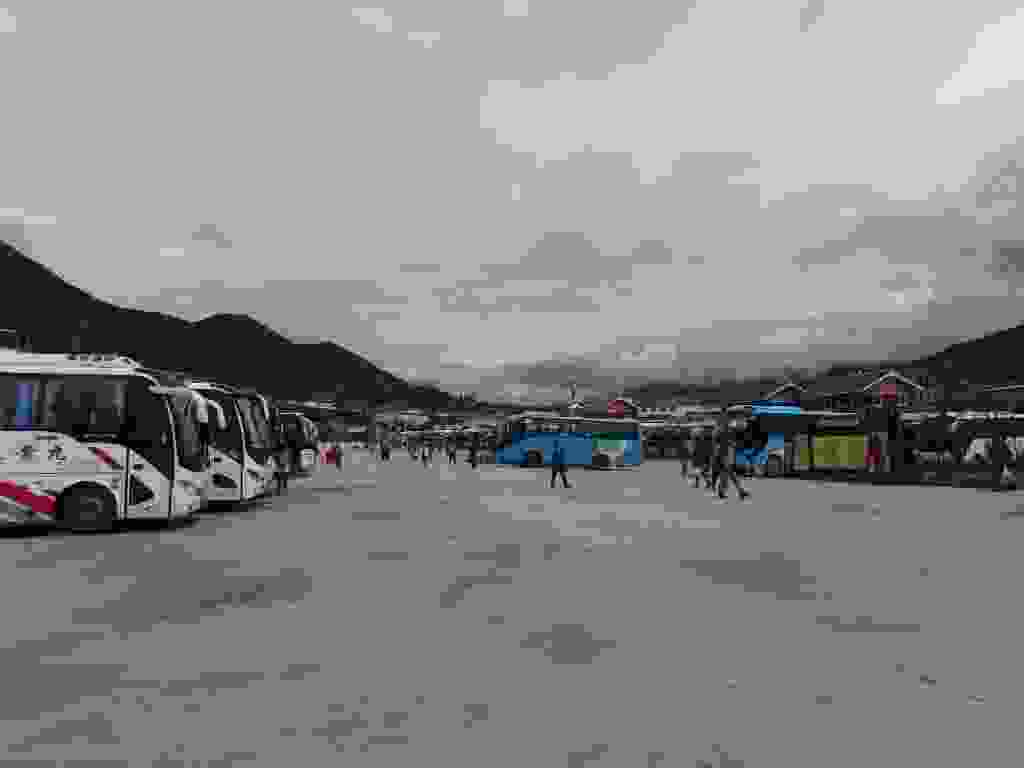
\includegraphics[width=\mywidth]{../wp-content/uploads/2015/09/wpid-p9176972-1024x768.jpg} \end{center}

 

 Passage obligé sur l'autoroute, une partie de la nationale n'a pas été reconstruite après le tremblement de terre de 2008 

 

\begin{center} 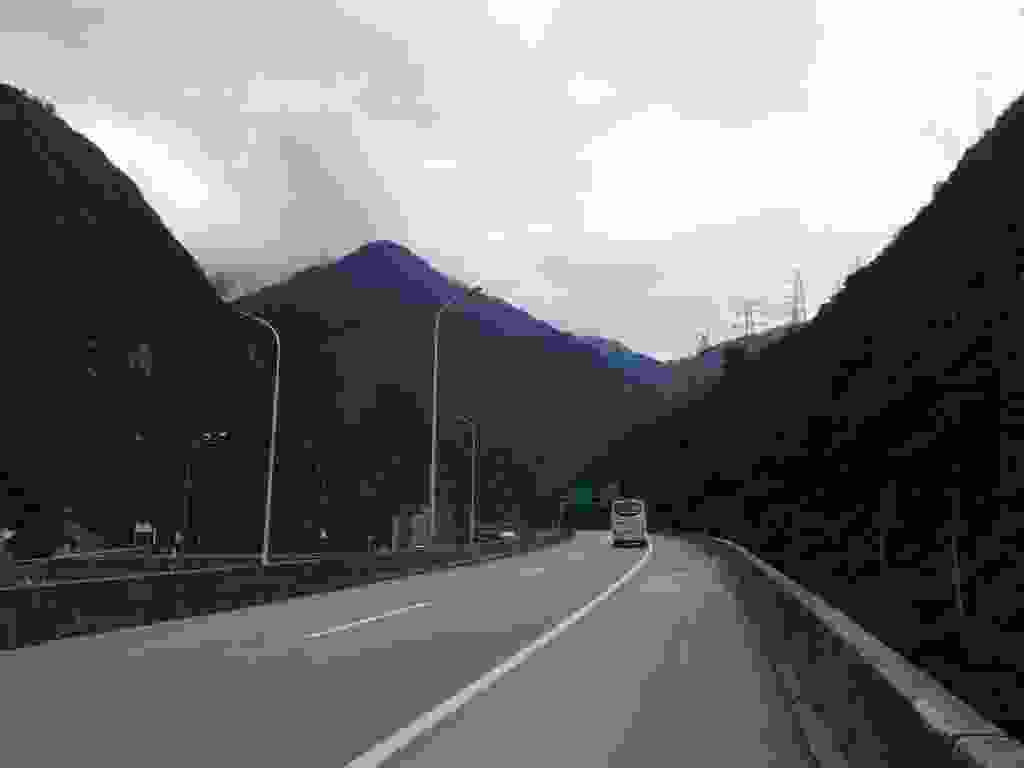
\includegraphics[width=\mywidth]{../wp-content/uploads/2015/09/wpid-p9197010-1024x768.jpg} \end{center}

 

 

\begin{center} 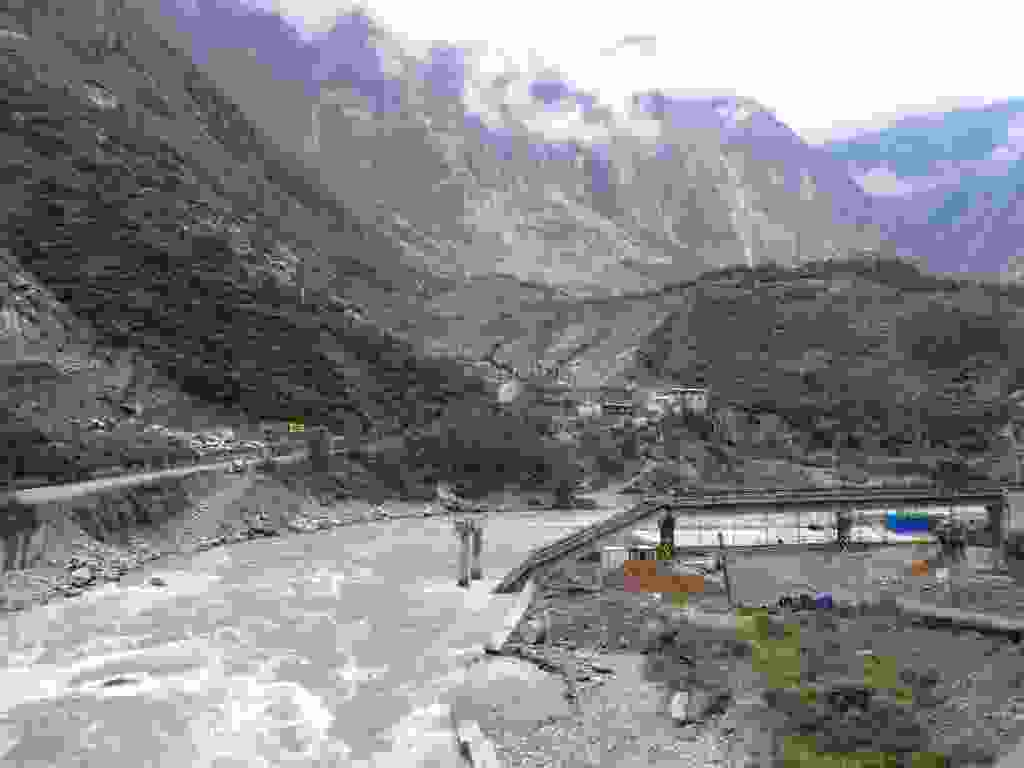
\includegraphics[width=\mywidth]{../wp-content/uploads/2015/09/wpid-p91970091-1024x768.jpg} \end{center}

 

 

\begin{center} 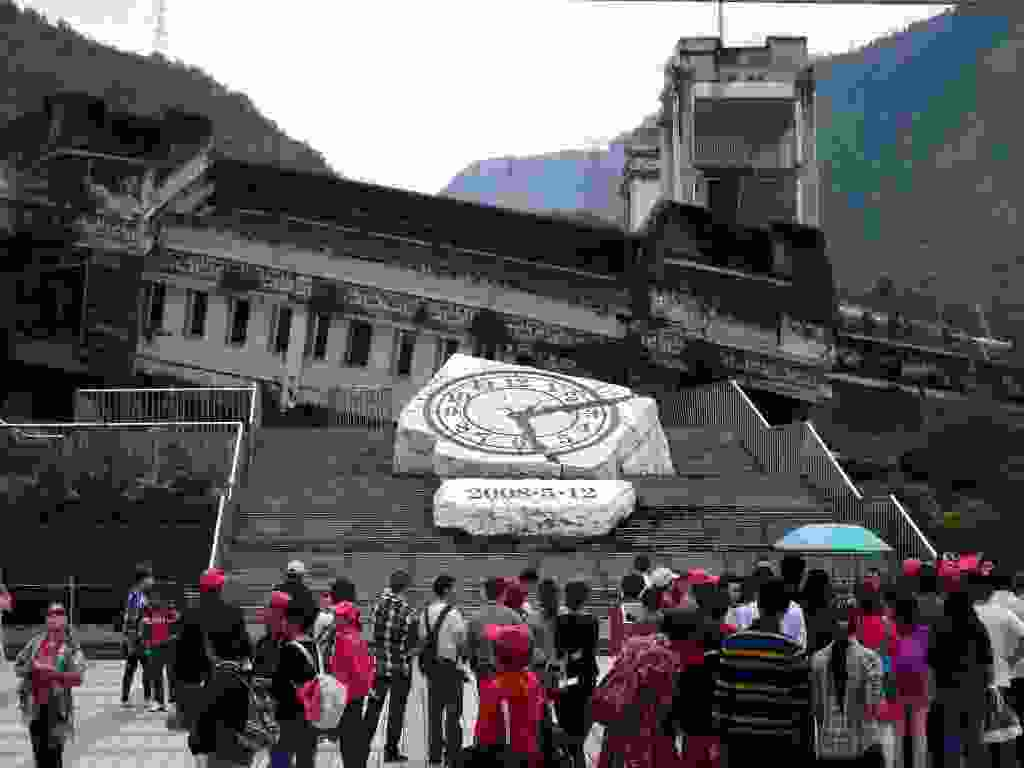
\includegraphics[width=\mywidth]{../wp-content/uploads/2015/09/wpid-p91970121-1024x768.jpg} \end{center}

 

 Contournement d'un grand lac avant d'arriver à Dujiangyian 

 

\begin{center} 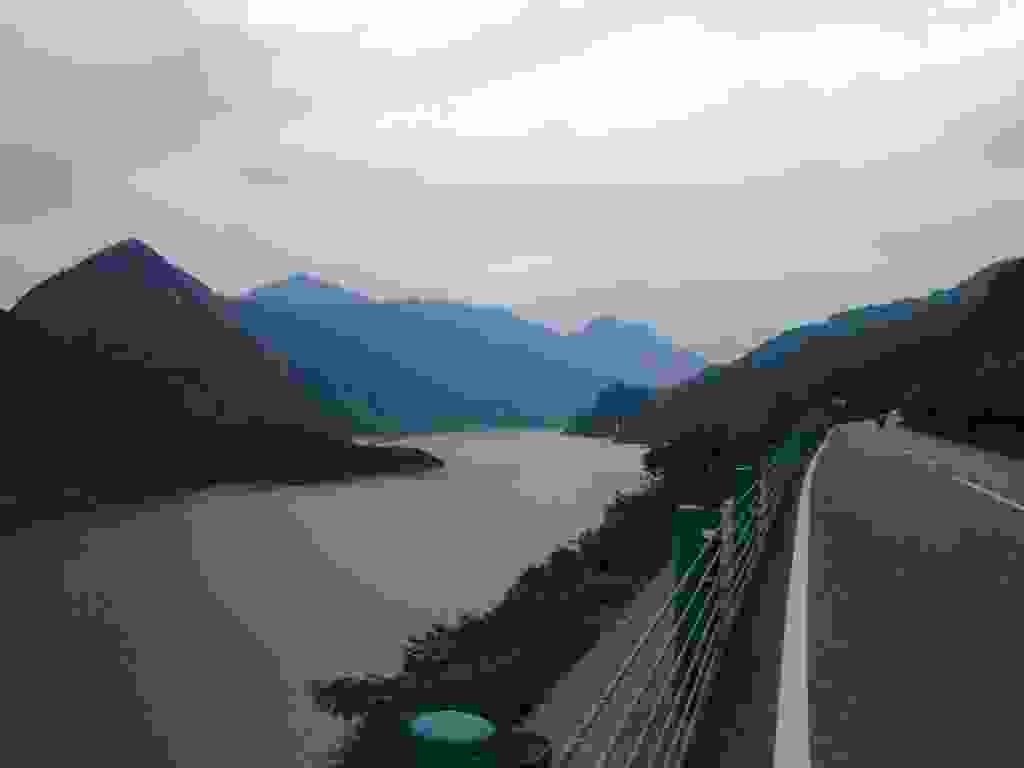
\includegraphics[width=\mywidth]{../wp-content/uploads/2015/09/wpid-p9197016-1024x768.jpg} \end{center}

 

 

\begin{center} 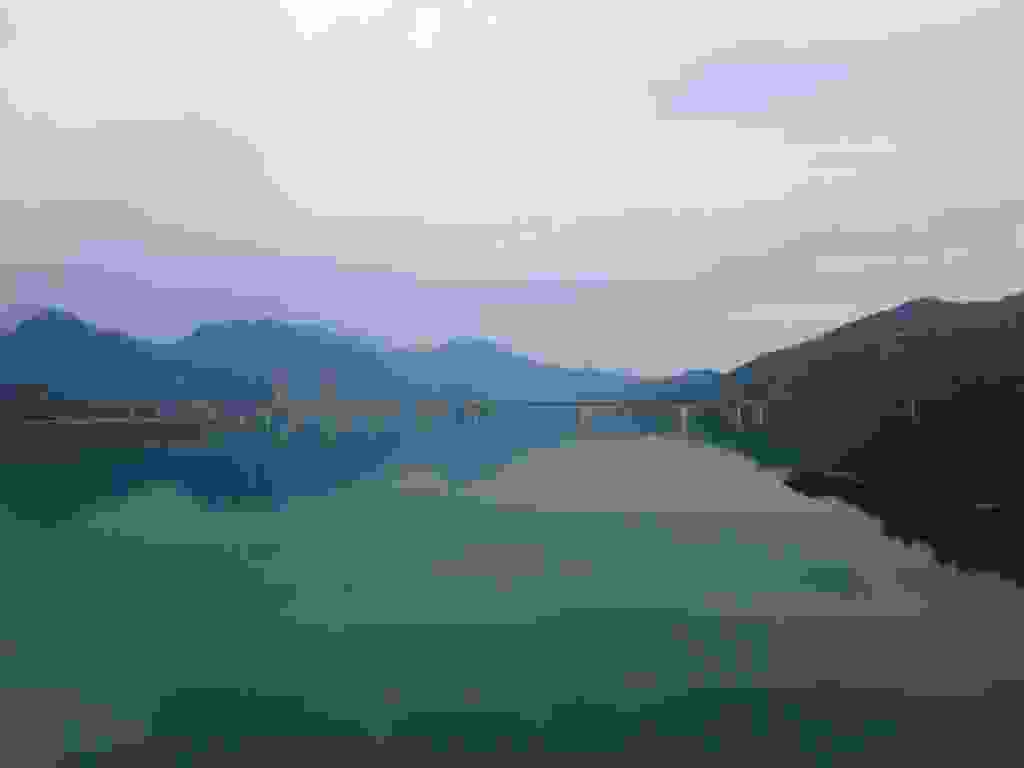
\includegraphics[width=\mywidth]{../wp-content/uploads/2015/09/wpid-p91970172-1024x768.jpg} \end{center}

 

 Je visite le système d'irrigation de Dujiangyian construit il y a plus de 2000 ans 

 

\begin{center} 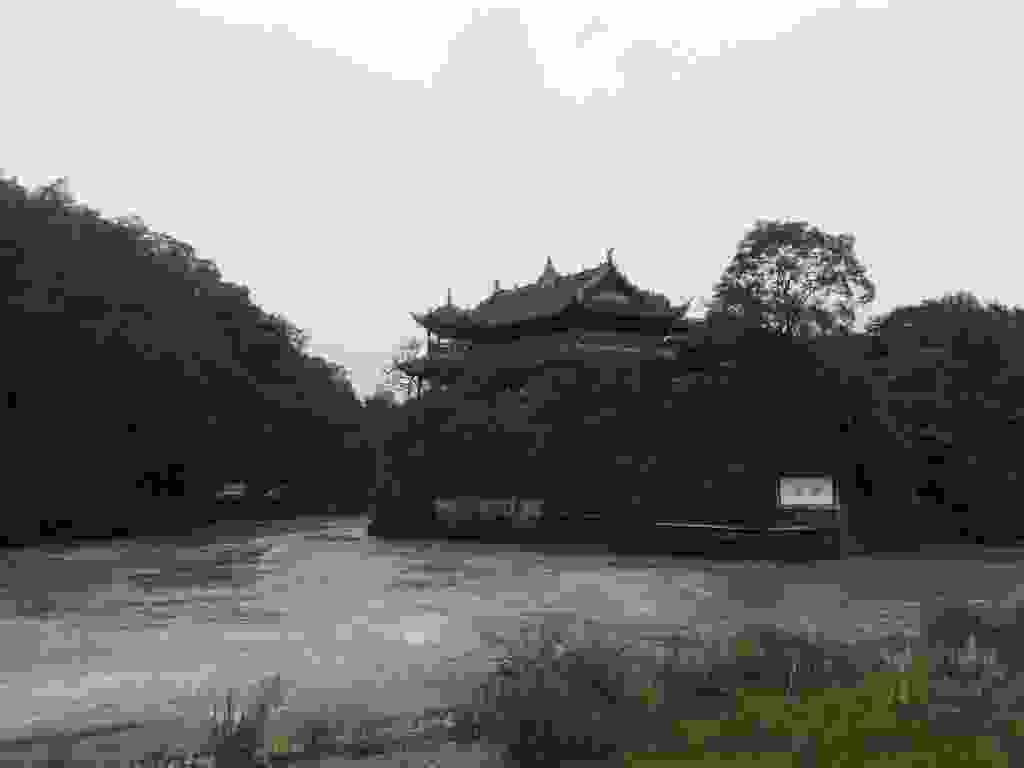
\includegraphics[width=\mywidth]{../wp-content/uploads/2015/09/wpid-p9207025-1024x768.jpg} \end{center}

 

 

\begin{center} 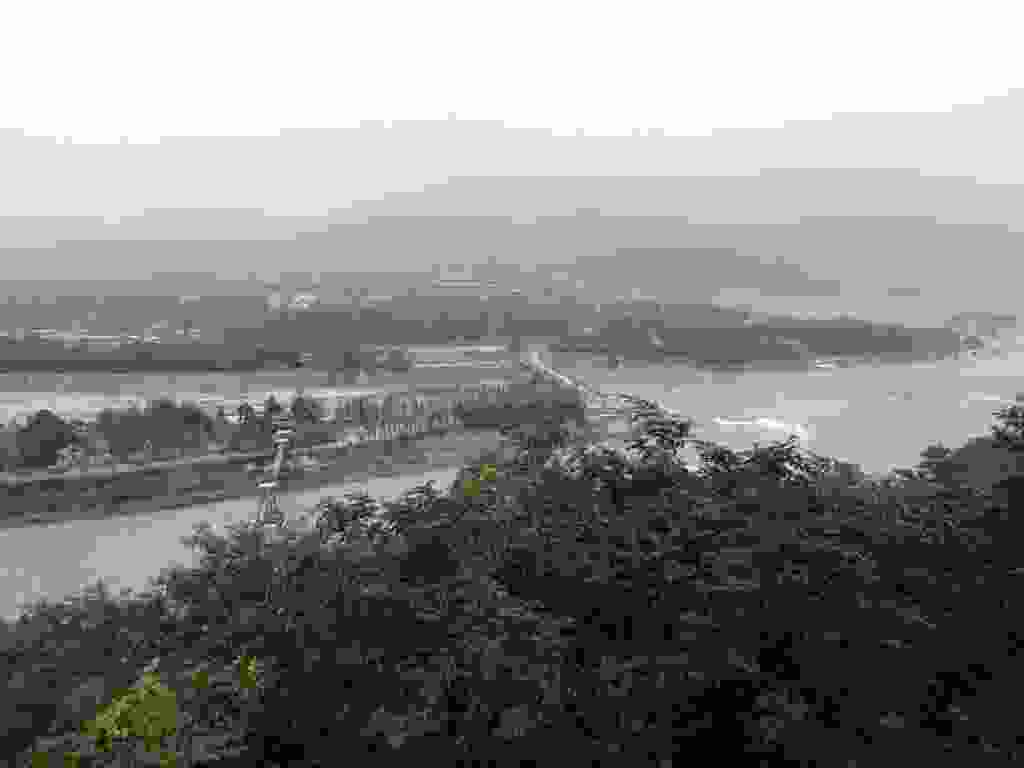
\includegraphics[width=\mywidth]{../wp-content/uploads/2015/09/wpid-p9207031-1024x768.jpg} \end{center}

 

 

\begin{center} 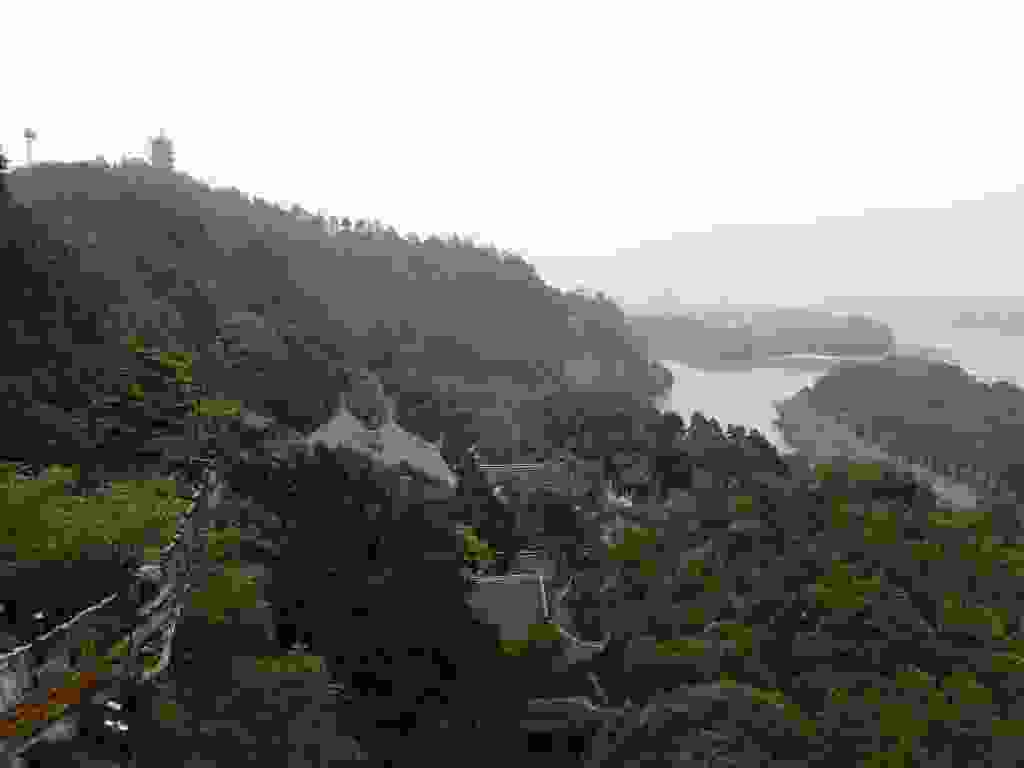
\includegraphics[width=\mywidth]{../wp-content/uploads/2015/09/wpid-p9207032-1024x768.jpg} \end{center}

 

 A quelques km le mont Qingcheng et ses temples taoïstes, il faisait vraiment moche je me suis contenté du premier temple en bas 

 

\begin{center} 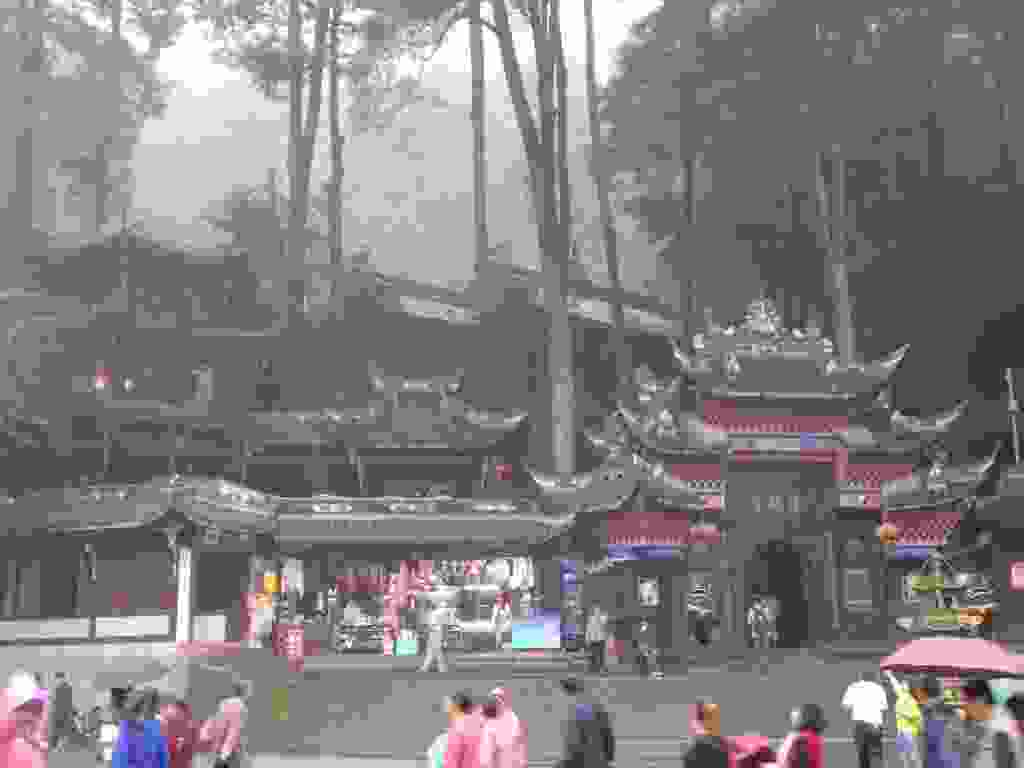
\includegraphics[width=\mywidth]{../wp-content/uploads/2015/09/wpid-p9207048-1024x768.jpg} \end{center}

 

 

\begin{center} 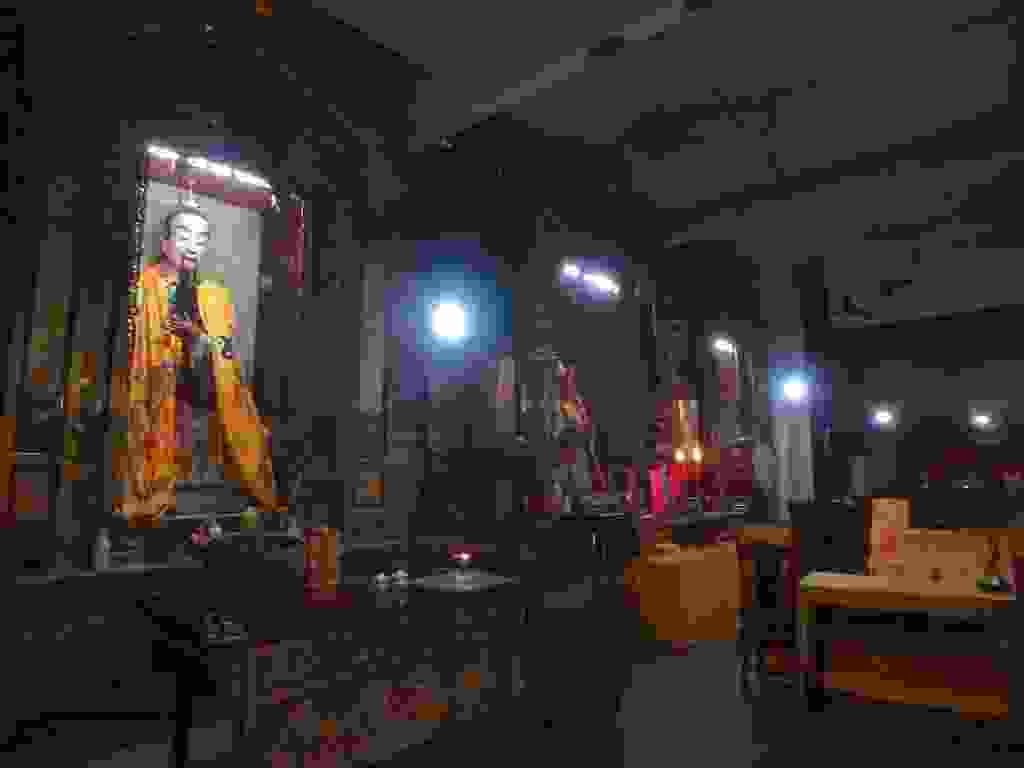
\includegraphics[width=\mywidth]{../wp-content/uploads/2015/09/wpid-p9207047-1024x768.jpg} \end{center}

 

 Les pandas, symboles du Sichuan, à l'entrée de Chengdu 

 

\begin{center} 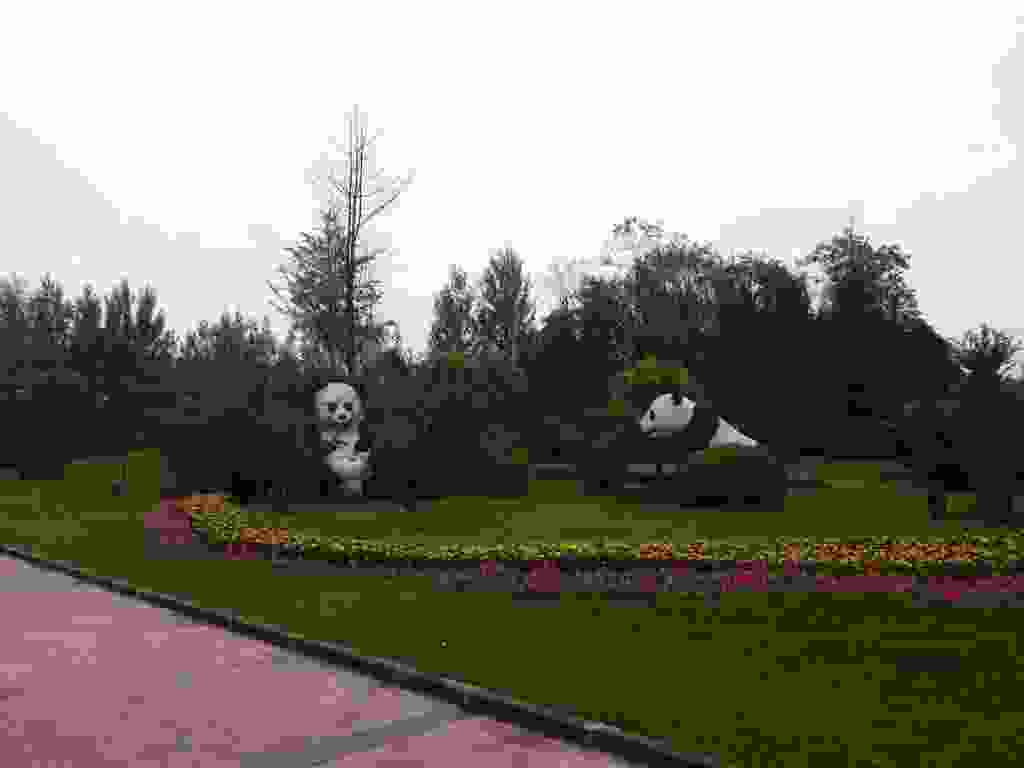
\includegraphics[width=\mywidth]{../wp-content/uploads/2015/09/wpid-p92170512-1024x768.jpg} \end{center}

 

 Cuisine bien pimentée dans le Sichuan, plat à base de poulet et cacahuètes que j'ai retrouvé plusieurs fois 

 

\begin{center} 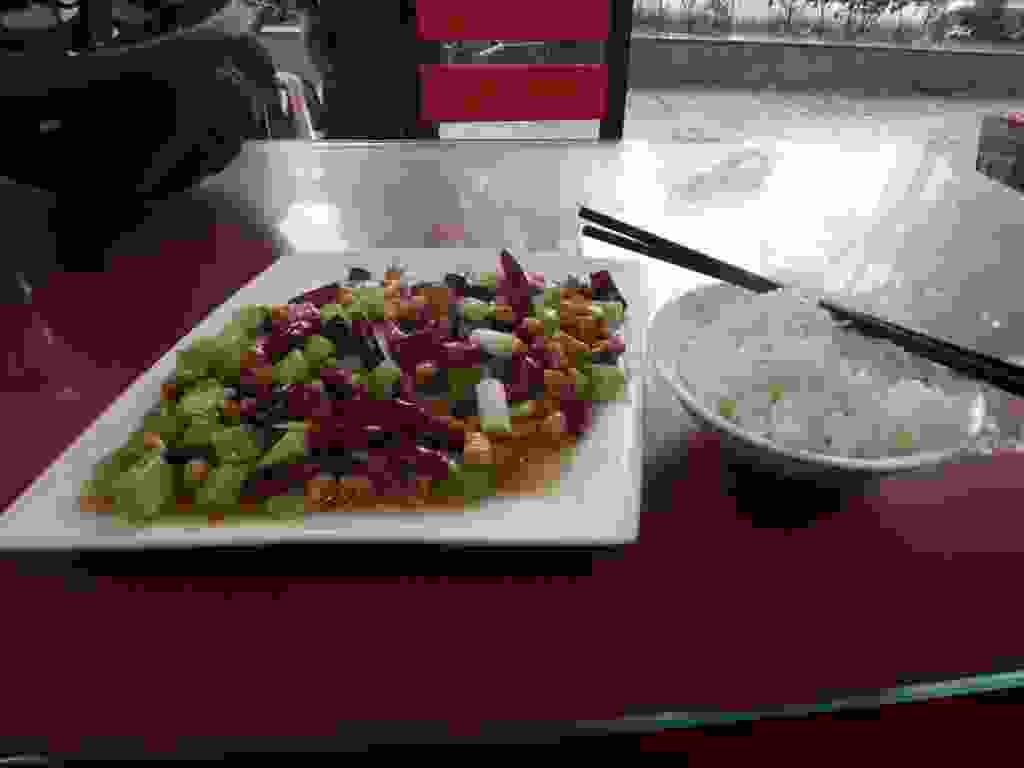
\includegraphics[width=\mywidth]{../wp-content/uploads/2015/09/wpid-p9207045-1024x768.jpg} \end{center}




 
 
